\section{Discussion of risks and opportunities} 
\label{sec:risks_opps}
%Having gestured towards our \textit{wants} inside and outside of exoplanets, and how different extended missions might or mightn't help address them, we turn now to discuss what we see as certain opportunities, as well as risks, that come from each extended mission scenario.
%A few of the opportunities we present overlap with our broader desires in exoplanet science -- for instance, an important reason to observe the \kepler field would be to measure transit timing variations.
This section begins to answer the question ``what opportunities will extended mission \textit{X} give?''.
%Section~\ref{sec:broader_science_beyond_planet_detection_stats}, conversely, began to discuss the question `what are our desires inside and outside of exoplanet science?'.
Most of the following points entail considering \tess in its broader context, rather than focusing only on what the \tess instrument itself is capable of observing as we did in Sec.~\ref{sec:broader_science_beyond_planet_detection_stats}.
%Perhaps the question we are actually trying to get closer to is ``how do we use \tess in order to maximize its astrophysical potential?''

%Aside from non-transiting-planet-oriented stuff, there's still a bunch of transiting-planet-oriented stuff that we need to discuss.

\subsection{Opportunities}
\paragraph{What's best on a $>1$ year horizon for planet detections?}
% Contextualize importance of thinking beyond just 1 yr extended mission
\tesss orbit is stable for more than 1000 years~\citep{gangestad_high_2013}.
While minor mechanical failures should be expected on the timescale of a few years, it is plausible that the spacecraft could outlive both the 2-year primary mission and the 1-year extended mission.
It is therefore important to select a 1-year extended mission scenario that offers strong prospects for continued observing.

% Preliminary discussion of immediate extensibility
A simple point is that \nhemi, \npole, and \shemiAvoid\ can all be inverted to their southern or northern complements for a fourth year of observing.
This will yield a comparable number of new planets to what they find in year 3 ($\mathcal{O}(1300)$ with $R_p<4R_\oplus$).
This argues strongly to continue observing the entire sky, rather than focusing on a single ecliptic hemisphere after the primary mission's completion.
This would continue \tesss role as a planet-discovery machine, while also addressing the practical matter of refining ephemerides in order to enable detailed characterization with suitable instruments.
%Leave the detailed characterization for \jwst, Spitzer, HST, ground-based ELTs, and posterity.

The \elong, \eshort, and \hemis\ scenarios are less obviously extensible to multiple years.
The main reasons to return to the ecliptic after performing \elong\ or \eshort\ would be to make \tesss survey truly `all-sky', and to complete all possible \ktwo follow-up observations (see discussion below).
Of course, this would need to happen during intervals in which the Moon and Earth were not in the way.
%Continuous observations have serious value. 

% Move on to very-long term comments.
Any of our proposed scenarios could simply be repeated indefinitely (as could their two-year `all-sky' versions).
%The `continuous viewing zone' in this scenario would fundamentally change: instead of having 1 year of continuous \tess data on a given star in the CVZ, we would have data with a 1-year baseline and a 14-day window function, and for twice as many stars.
The main trade-off this presents becomes apparent comparing 2 years of \hemis\ to repeating the primary mission over 2 years.
If we repeat the primary mission over 2 years, the northern and southern CVZs each get 1 year of continuous observation.
If we do \hemis\ for 2 years, the northern and southern `long viewing zones' each get 2 years of 14-day windowed observations.
The latter case allows 2-transit detections of $P\lesssim1$ year planets over $2\%$ of the sky.
The former allows 2-transit detections of $P\lesssim6$ month planets over $1\%$ of the sky.
This simple consideration of course misses that point that data obtained from repeating the primary mission would be less subject aliasing issues and would have fewer period ambiguities.
That said, repeating \hemis\ for two years might be a middle ground between a strategy like ``repeat \npole\ indefinitely'' and ``repeat the primary mission indefinitely''.

%That said, the latter would only allow for planets to be detected with periods twice as long!

A longer-term question is ``when will \tess hit the point of diminishing returns?''
The `low-hanging fruit' of small planets transiting bright stars at short orbital periods will eventually be found if \tess continues to observe the same sky.
The most important qualitative point of this memo, made in Fig.~\ref{fig:snrf_histogram}, is that after \tesss primary mission there will be many objects remaining for which merely doubling the number of observed transits will enable their detection.
Eventually though, the peak of the phase-folded SNR distribution shown in Fig.~\ref{fig:snrf_histogram} will shift past the detection threshold, and more observations will only allow us to probe out to longer orbital periods and dimmer stars.
No detailed study has yet quantified when \tess will reach this inevitability.
%We're not really sure when we're going to reach this regime.

However, we can use \kepler's primary mission as a point for comparison: we retrieve all KOIs with a Kepler Disposition of `CANDIDATE' as reported by NASA's Exoplanet Archive (August 15, 2016), and plot the periods of KOIs as a function of KOI number, coloring each KOI by its radius.
\todo[inline]{did kepler actually reach this regime? ask J Rowe? maybe want same plot, colored by kep mag too? this \& above paragraph maybe cut...}
If we take the KOI number as a rough proxy for total observing time of a given \kepler object (ignoring short-term sociological trends), if \kepler reached the `point of no more low-hanging fruit', we would expect the later KOI numbers to not have any short-period small planets.
Fig.~\ref{fig:kepler_diminishing} shows that even after 4 years of observing the same field, the \kepler team was still announcing short-period small planet detections.
Given this result it seems likely that \tess could perform a scenario like \nhemi\ or \npole\ for $>2$ years before this became an issue.
\begin{figure*}
	\centering
	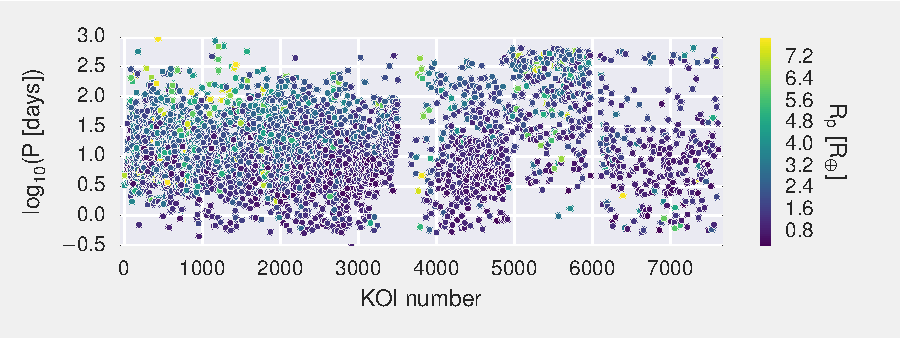
\includegraphics[scale=1.]{figures/kepler_diminishing.pdf}
	\caption{ Did \kepler reach the point of diminishing returns? The first catalog went up to KOI number 1000. Q6 took us to 2000, Q8 to 2800, Q12 to 4200, Q16 to 5500, and Q17 (DR24) to 7000.
		The pipelines changed in these times (Q6 pipeline method for single pass detections, multis from BLS, Q8 switch to multiple-pass wavelet, Q12 to community disposition, Q16 to automating disptions, Q17 to robovetting and deep EBs)}
	\label{fig:kepler_diminishing}
\end{figure*}


\paragraph{Ability to upgrade cadence of targets detected in long-cadence images}
How adept will we be at upgrading suspected transiting planet hosts to shorter cadence?
This is an issue relevant to both \tesss primary mission as well as the extended mission:
if it becomes apparent from the SPOC's processing that a FFI transit-signal in the $N^\mathrm{th}$ observing sector is likely a planet, it could be observed at short cadence in the $(N+1)^\mathrm{st}$ observing sector to improve the probability both of detecting a planet, and also of obtaining a detection with precise orbital parameters.
Adding such stars will not crowd-out a significant number of stars from the baseline target list provided that a strong enough threshold is set for what becomes labeled a `promising candidate'.
As planned, the SPOC will only compute pixel-level calibrations, and not light curves, from the FFI data~\citep{jenkins_SPOC_2016}.
A `quick-look' FFI pipeline could be an important tool towards optimizing \tesss science yield based on this point.
\todo[inline]{so they're not doing ANY planet candidates?}

Our simulation ignored this question and assumed that \textit{none} of the planets or planet-candidates found in the primary mission would be observed at upgraded cadence, unless when their star's \texttt{Merit} was recomputed for the extended mission, it happened to rank in the top $2\times10^5$ targets.
Another extreme would be to upgrade \textit{every} TOI from the primary mission to 2 minute cadence in an extended mission.
If we did this, one major change in our predicted yield would be that Fig.~\ref{fig:yield_results} would show nearly all of the extended mission's `new planets' being detected in postage stamps. 
More importantly, this strategy would lead to more planet detections by helping build SNR on transiting events with $\lesssim1\ \mathrm{hr}$ durations, and also potentially help in detecting additional transiting companions. 
%since most of the newly detected planets in an extended mission are objects that transit during the primary mission (and thus that would hopefully make the TOI list).


\paragraph{Modify the cadence for full frame images and target stars; modify allocation of data mass between them.}
The above question on upgrading the cadence of promising targets ties into a broader question: ``what is the optimal cadence and relative weight between postage stamps and full frame images?'' 
%\todo[inline]{fix the title of this figure.}
To our knowledge, this question has not been studied in depth.
By way of preliminary calculation, we ran our yield simulation for the primary mission, but rather than observing $2\times10^5$ 2-min targets and $3.8\times10^6$ 30-min targets, we observed $4\times10^5$ 4-min targets and $3.6\times10^6$ 30-min targets (note both cases that the FFIs are complete for $R_p<4R_\oplus$).
This simple change increases the absolute number of detected planets by $\sim$15\%.
\begin{comment}
We show the yields in Fig.~\ref{fig:400k_at_2min}. 
This simple change improves the planet detection yield by $\sim15\%$ (compare with Fig.~\ref{fig:primary_planet_yield}).
\begin{marginfigure}
	\centering
	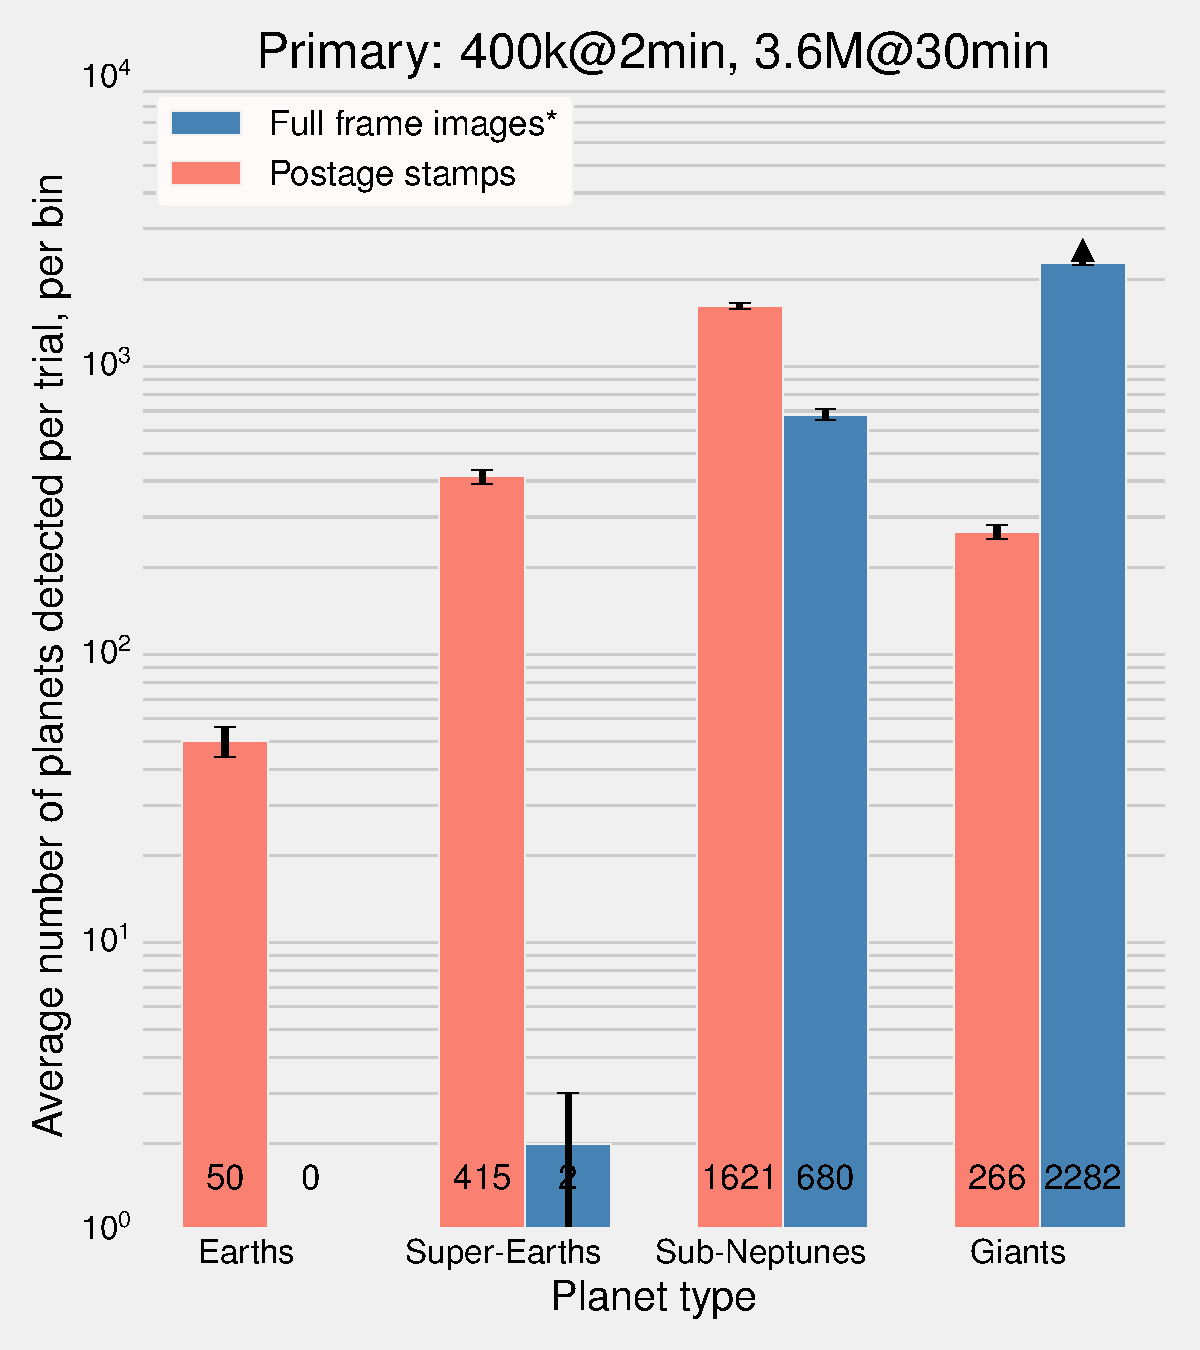
\includegraphics[scale=1.]{figures/160816_400k_at_4min_36M_at_30min_shemi_nhemi_nhemi_t20-pri.pdf} % it's actually 400k at 4minutes!
	\caption{The yield from running the primary mission with the top $4\times10^5$ ranked \texttt{Merit} stars at 4 minute cadence, and then next $3.6\times10^6$ at 30 minute cadence. The absolute yield improves relative to the nominal 200k\@2min, 3.8M\@30min (Fig.~\protect\ref{fig:primary_planet_yield}) by a factor of $\sim1.15$.}
	\label{fig:400k_at_2min}
\end{marginfigure}
\end{comment}

The main benefit of short cadence in transit detection is in resolving the shortest transit durations that would otherwise be `smeared'.
30 minute cadence is sufficient for this purpose on most transit timescales (with the exception being the closest planets to M dwarfs).
Auxiliary benefits of shorter cadence include: \textit{(a)} resolving the ingress and egress phases of transits, which helps remove degeneracies during retrieval of a planet's physical and orbital parameters, and \textit{(b)} retrieving precise mid-transit times and ingress/egress times, which helps ephemeris prediction.
%   * Look at Carter+Winn (2008), or Price+Rogers (2014) [who do the same thing w/out a trapezoidal approxn
%   --> can be ~an OOM better precision for uncertainty on ingress/egress time, and factor of
%   ~3 better for uncertainty on mid-transit time (2min vs 30min, rough guess; Price+Rogers 2014;  abstract cites 30min vs instantaneously-sampled).
   
%   * From "brute force" approach:
%   * Numbers in email likely fine: 2->15min drop by factor ~1.1 in planet yield across the board;
%   2->30min drop by factor ~1.2. (Ignores worse uncertainties on parameter retrieval)

While 2 minute cadence may be overkill for simply detecting transits, the benefits that come from fine time-resolution may justify the additional data cost.
That said, we may discover in the primary mission (or beforehand, if this question is studied at greater depth) that 2 minute cadence is not worth the additional cost; in that case, we could change these parameters in an extended mission.


\paragraph{Follow-up for \tess:}
Ground and space-based instruments will reveal essential details of the \tess planet sample.
Given the impracticality of listing out every such facility, we focus here on the resources that we expect will be most important towards broadly advancing our understanding of \tesss planets.

\begin{itemize}
	\item \textit{\jwst:}
	Exoplanet observations with \jwst will encompass transit, occultation, and phase curve measurements.
	%The ideal planet for building a large SNR orbits a bright, photometrically stable host; large ratio of planet to star radius; large atmospheric absorbing areas, driven by high planet temperature, low planet surface gravity, and low mean molecular weight of planetary atmospheres for transmission spectroscopy; deep spectral absorption features; relatively high planet to star temperatures for emission observations; and short orbital periods for phase curve
	The class of measurement determines the planetary and stellar parameters that are most important in building a large SNR, but for all three classes of observation, many promising targets are already known~\citep{stevenson_communityJWST_2016}.
	The main contribution of \tess will be finding hitherto unknown sub-Neptune radius planets orbiting bright stars.

	The main point for consideration of \tess and \jwsts overlap is that of sky coverage.
	\jwst can observe targets within $5^\circ$ ($10^\circ$) [$60^\circ$] of the North and South Ecliptic Poles for the entire (two thirds of the) [one third of the] year.
	The feasibility of transit programs that require multiple visits, for instance super-Earth spectroscopy, thus greatly depend on their targets' on-sky locations.

	To assess how much extended \tess missions might actually impact this point of overlap, we ask:
	\textit{(1)} How many new $R_p<4R_\oplus$ planets does each scenario give in \jwsts easily-viewed zones? 
	\textit{(2)} Of those, how many have atmospheres prone to characterization?
	
	\afterpage{
\begin{longtable}{lrrrr}
\caption{Newly detected sub-Neptune radius planets.
	$|\beta|>85^\circ$ can be observed all year by \jwst\!;  $|\beta|>80^\circ$ can be observed for $\ge$ two-thirds of the year, $|\beta|>30^\circ$ for $\ge$ one-third.} \label{tab:jwst0}\\
\toprule
{} &  $|\beta|>85^\circ$ &  $|\beta|>80^\circ$ &  $|\beta|>30^\circ$ &  All sky \\
\midrule
primary    &                 103 &                 453 &                2088 &     2483 \\
\nhemi      &                  38 &                 170 &                1024 &     1284 \\
\npole      &                  41 &                 176 &                1419 &     1419 \\
\shemiAvoid &                  24 &                 100 &                 934 &     1327 \\
\elong      &                  22 &                  86 &                 667 &     1169 \\
\eshort     &                  12 &                  52 &                 857 &     1216 \\
\hemis   &                  44 &                 192 &                1130 &     1433 \\
\bottomrule
\end{longtable}
\begin{longtable}{lrrrr}
\caption{$R_p>4R_\oplus$ and $\mathrm{SNR_{atm}>SNR_{GJ\ 1214b}/2}$.} \label{tab:jwst1}\\
\toprule
{} &  $|\beta|>85^\circ$ &  $|\beta|>80^\circ$ &  $|\beta|>30^\circ$ &  All sky \\
\midrule
primary    &                   1 &                   4 &                  71 &      104 \\
\nhemi      &                   0 &                   0 &                   7 &       14 \\
\npole      &                   0 &                   0 &                   8 &        8 \\
\shemiAvoid &                   0 &                   0 &                   8 &       24 \\
\elong      &                   0 &                   0 &                   5 &       21 \\
\eshort     &                   0 &                   0 &                   9 &       23 \\
\hemis   &                   0 &                   0 &                  10 &       22 \\
\bottomrule
\end{longtable}
\begin{longtable}{lrrrr}
\caption{$R_p>4R_\oplus$ and $\mathrm{SNR_{atm}>SNR_{GJ\ 1214b}/5}$.} \label{tab:jwst2} \\
\toprule
{} &  $|\beta|>85^\circ$ &  $|\beta|>80^\circ$ &  $|\beta|>30^\circ$ &  All sky \\
\midrule
primary    &                  21 &                  83 &                1019 &     1361 \\
\nhemi      &                   1 &                   4 &                 242 &      397 \\
\npole      &                   1 &                   4 &                 278 &      278 \\
\shemiAvoid &                   1 &                   3 &                 261 &      523 \\
\elong      &                   1 &                   3 &                 164 &      445 \\
\eshort     &                   0 &                   2 &                 299 &      530 \\
\hemis   &                   1 &                   6 &                 312 &      515 \\
\bottomrule
\end{longtable}
} % source of data: jwst_tess_overlap_stats.ipynb, which processes the same files from the main yields presented (so 160729, t50).	
	
	We answer these questions in Tables~\ref{tab:jwst0} to \ref{tab:jwst2}.
	The glaring point of Table~\ref{tab:jwst1} is that there will be very few \tess\!-detected super-Earths in \jwsts continuous viewing zones with truly great prospects for transmission spectroscopy.
	This is a geometric problem (the \jwst CVZs take up $0.4\%$ of the sky) as well as an abundance problem (most $R_p<4R_\oplus$ planets have substantially less SNR in transmission than GJ 1214b).
	
	Another important trend from the tables is that while $|\beta|>80^\circ$ planets show a factor of 4 difference in yield between \eshort\ (50) and \hemis\ (200), if we restrict our interest to $\mathrm{SNR}_\mathrm{atm} > \mathrm{SNR}_\mathrm{GJ\ 1214b}/5$ planets, there is practically no difference between extended missions; the primary mission detects the most important planets for \jwst follow-up.
	
	Given that a $R_p<2R_\oplus$ planet must be observed in-transit for hundreds of hours to yield atmospheric temperatures and abundances of select molecules~\citep{gillon_trappist1_2016,barstow_trappist_2016}, it is likely that only the very best targets will be selected.
	That said, the main point of Table~\ref{tab:jwst2} is that \tess will detect the most promising planets for \jwst follow-up after only a year's observation.
	This means that \tess is not `bound' to the ecliptic poles in an extended mission to support \jwsts target selection.
	More important for ensuring \jwst\!--\tess overlap will be the efficient spectroscopic and photometric follow-up of \tesss planets from the ground; by \jwsts launch in October 2018, only a few verified \tess planets will be known.
	
	In passing, we highlight an important assumption relevant to this topic: our \texttt{Merit} statistic is weighted by $\sqrt{N_\mathrm{obs}}$, so our density of target stars near the ecliptic poles is roughly $3.5\times$ that nearest to the ecliptic plane.
	The actual prioritization scheme for \tess targets may differ.
	An additional minor concern is the saturation limits on \jwsts instruments -- $J \gtrsim 6$ ($J>11$) for medium (low) resolution NIRSpec spectroscopy, and $J > 8.1$ ($J>6.9$) for standard (subarray) spectroscopy with NIRISS~\citep{beichman_observations_2014}.
	Only a small number of \tesss planets reach these limits.
	
	\item \textit{CHEOPS:}
	We refer the interested reader to~\citet{berta_cheops_2016} for an overview of how \tess and \cheops complement each other.
	Re-stating the main points:
	\cheops provides more precise photometry for essentially all stars than \tess, and uses a narrow field of view to select individual targets.
	\cheopss visibility is best near the ecliptic, and non-existent near the ecliptic poles.
	\tess and \cheops could together measure TTVs, to both measure planet masses and also search for additional companions. 
	As these systems will be accessible to radial velocities, they will be important keystones for cross-checking RV and TTV mass measurements.
	
	Extended missions that focus exclusively on the ecliptic poles, like \npole, seriously neglect the complementarity of \tess and \cheops\!.
	Those that focus on the ecliptic, including \elong\ and \eshort, provide the largest amount of overlapping coverage.
	
	
	\item \textit{Ground-based follow-up for \tess:}
	Ground-based spectroscopic and photometric follow-up are essential components of \tesss baseline mission.
	After rejecting false-positives probabilistically or via imaging and reconnaissance spectroscopy, RV measurements will yield masses and orbital elements, \textit{e.g.,} eccentricities, for many \tess planets.
	Ground-based supporting photometry taken before, during, and after \tesss observations will also help in discovering longer period companions to short-$P$ transiters, and in building SNR on $R_p\gtrsim4R_\oplus$ planets.
%	\todo[inline]{possibly support based on Gaspar's or Maximilian's predictions}
	
	The primary mission will clarify whether ground-based follow-up resources need to constrain \tesss extended observing.
	Based on the expected contributors for RV as well as photometry -- HARPS, HARPS-N, CARMENES, SPIROU, LCOGT, HAT, KELT, WASP, NGTS, and others -- there should be ample resources in both hemispheres for \tess to be able to observe anywhere without risking insufficient follow-up.

	That said, a minor bonus for focusing \tess observations near the ecliptic as in \elong\ or \eshort\ is that relatively more ground-based telescopes can follow-up on these targets, rather than only those in Earth's northern or southern hemispheres.
	
	An additional point to be considered for ground-based follow-up of an extended mission would be to confirm \tess planets orbiting rapidly rotating stars through spectroscopic transit measurements of the Rossiter-McLaughlin effect \textit{e.g.},~\citep{gaudi_prospects_2007}.
	Multiplexing spectrographs might enable confirmation (without mass measurements) at a more rapid rate than measuring the orbital velocity of the parent star over a full orbital period.
	
	% DO CONTEMPORANEOUS OBSERVATIONS HAVE VALUE AS WELL?
\end{itemize}




\paragraph{TESS as a follow-up mission}
\label{par:TESS_as_followup}

Hundreds of transiting exoplanets have been discovered from the ground\footnote{Notably surveys %and telescopes 
	that have discovered transiting planets % after HD209458's discovery~\citep{charbonneau_detection_2000,henry_transiting_2000} 
	include OGLE~\citep{udalski_ogle0_2003,udalski_ogle1_2003}, HAT~\citep{bakos_HAT_2004}, TrES using STARE~\citep{alonso_tres1_2004}, the XO telescope~\citep{mccullough_xo_2005}, WASP~\citep{pollacco_wasp_2006}, KELT~\citep{pepper_KELT_2007}, MEarth~\citep{irwin_mearth_2008}, TRAPPIST~\citep{jehin_trappist_2011}, and the Qatar Exoplanet Survey (QES)~\citep{alsubai_qatar_2014}. Other transit surveys have recently begun: the APACHE project observes from the Western Italian Alps~\citep{sozzetti_apache_2013}; SPECULOOS will soon begin observing from the Atacama Desert~\citep{gillon_speculoos_2013}; NGTS is succeeding SuperWASP~\citep{wheatley_ngts_2013} }
and thousands have been found from space.
\tess will follow-up on these discoveries -- the primary mission's target list will include known planet-hosts from transit and RV surveys.
While the value-added will be largest for systems that only have ground-based photometric and/or spectroscopic data, % and refine with space-based transits.
many of these systems could yield additional transiting companions along with refined physical and orbital parameters for the known planets.
An inspiring example is the WASP-47 system, for which the WASP team found a hot Jupiter, subsequent RV follow-up yielded a $P=2$ year Jupiter-mass outer companion, and further \ktwo observations yielded two $R_p<4R_\oplus$ planets transiting inside and outside of the hot Jupiter's orbit~\citep{hellier_wasp47_2012,neveu-vanmalle_HJrelatives_2016,becker_wasp47_2015,dai_doppler_2015}.
Even for the \kepler field, which \tess will observe with less precision than \kepler had, \tesss observations will aid analyses of transit timing variations, secure a small number of long-period transiters, and provide a cross-calibration between the two missions.	

We highlight where we expect \tess to provide a substantial additional value to already-studied fields and systems:
%Rather than list every transit survey and perform a detailed analysis of what it learned, and what we can learn with TESS that might different from what it learned, we focus on regions of the sky that have been targeted by various surveys, and note possible `value-added' where applicable:
\begin{itemize}
	\item \textit{Kepler's field:}
	\tess will observe the \kepler field for an average of $2\times26=52\ \mathrm{days}$ in 2019.
	This will also entail observing a few of \keplers modules for 78 days, and a few for 26 (see Fig.~\ref{fig:positions_pointings}).
	%\todo[inline]{what month? could ask jacobi, but it's extraneous}
	A practical note for extended missions is that \npole\ observes the \kepler field for an average of $4\times26=104$ days per year -- twice as long as \nhemi.
		
	The main reasons to allocate extra pixel weight to the \kepler field include:
	\textit{(a)} detecting transits over a long baseline (\textit{e.g.,} to refine ephemerides);
	\textit{(b)} measuring transit timing variations;
	\textit{(c)} confirming few-transit KOI candidates, \textit{e.g.}~\citep{wang_longP_2015,uehara_transiting_2016,foreman_mackey_longP_2016}, 
	\textit{(d)} calibrating \tess against well-studied candidates,
	\textit{(e)} continue observations of CBPs \& multiple star systems, and
	\textit{(f)} characterize stellar cycles over long timescales through star-spot measurements.
		
	\citet{sullivan_KOIs_2013} explored \tesss performance on KOIs in some detail.
	He found that even with \tesss reduced sensitivity to \keplers dim stars, it should detect $5-10\%$ of the KOIs at $\geq3\sigma$ significance per transit.
	A few dozen of these planets have $R_p<4R_\oplus$, and $\sim$50 reside in multi-planet systems and are likely to give interesting TTV measurements.
	We note that \citet{sullivan_KOIs_2013} used October 2013's KOI list, which has since at least doubled in length.
	
	\item
	\textit{Ground-based surveys:} 
	\tesss photometric precision provides the greatest relative benefit for planets that have never been observed from space.
	WASP and HAT have detected the largest number of transiting systems from the ground, in both the northern and southern celestial hemispheres.
	These targets, and even those from RV surveys, are promising candidates for detailed study in \tesss data.
	At the very least, \tess data for known transiters will yield improvements on uncertainties in planetary radii, and will also lead to discovery of many new transiting companions.
	Beyond transit science, the discovery of short-period non-transiting planets through phase curve measurements is also worth pursuing~\citep{millholland_detection_2016}.
	
	Will the desire to follow up ground-based surveys impact \tesss extended mission?
	Likely not; the north and south skies have similar numbers of known transiting and RV-detected planets.
	As long as the extended mission continues to observe both hemispheres (rather than focusing on a single one in perpetuity), the value-added to known transiting and even RV planets from the primary mission will only improve in an extended mission.

	\item \textit{K2:}
	\ktwo observes $\pm6^\circ$ about the ecliptic for $\sim$80 days per field, and is expected to discover anywhere from 500-1000 planets over its total mission lifetime~\citep{howell_k2_2014,crossfield_197_2016}.
	In a sense, \ktwo is a stepping stone between \kepler and \tess\!: \kepler observed a single field over a long baseline, \ktwo observes many fields over mid-length baseline, and \tess will observe the majority of the sky for a short baseline.
	
	If everything works, in early 2020 \tess will begin its extended mission and \ktwos on-board fuel supply will be either almost or entirely depleted.
	\ktwo will have covered $\gtrsim60\%$ of the area in the $|\beta|<6^\circ$ band about the ecliptic -- the exact band that \tess misses during its primary mission.
	Hundreds more \ktwo planets will be confirmed and vetted beyond those that already have been from early campaigns~\citep{foreman-mackey_k2_2015,vanderburg_234_2016,crossfield_197_2016}.
	% ALSO Kruse et al., in prep
	
	Our presentation of `newly detected planets' for both \elong\ and \eshort\ assumed no knowledge from \ktwo\!.
	This is quite unrealistic -- a large fraction of the planets that \tess will be capable of detecting near the ecliptic will already either exist as candidates in \ktwos data or have been discovered.
	Once processed, \ktwos precision is within a factor of 2 or 3 of \keplers\!; this is comparable to or better than \tess for most stars.
	%{is this true? i've never seen a plot comparing the photometric precision for all three missions. could add CHEOPS too (and a mission-switch option, for comparison)} 
	The median \ktwo candidate magnitude is 2 \kepler magnitudes brighter than that of KOIs\footnote{$K=12.8$ to $K=14.6$, based on data from NASA's Exoplanet Archive, August 21 2016} -- \tess would want to observe many of the same targets that are already being selected from the Ecliptic Plane Input Catalog~\citep{huber_epic_2016}.
	For a scenario like \elong, the average \tess coverage per star over the extended mission in the $\pm12^\circ$ band would be $\sim$7 spacecraft orbits, or $\sim$91 days of near-continuous observing.
	
	Summarizing then what we find to be the most compelling reasons to observe the ecliptic in an extended \tess mission:
	\textit{(a)} catch `holes' in the $|\beta| < 12^\circ$ band that \ktwo missed, completing the all-sky search for small planets transiting the brightest stars;
	\textit{(b)} observe targets in \ktwo fields that simply were not selected in \ktwos $\sim$20000 per campaign. For instance, \tesss bandpass allows probing down to cooler M dwarfs than \keplers\!;
	\textit{(c)} double the \ktwo observing baseline for most targets. In turn, confirm low-SNR candidates, and detect extra transits for a relatively large number of $20<P<40$ day planets;
	\textit{(d)} measure TTVs for targets over baselines up to 5-years.
	\textit{(e)} confirm a small but significant number of $P>40$ day planets (even single transiters, \textit{e.g.,}~\citep{osborn_single_2016}).

	\tesss value-added for the \ktwo targets is closer to that for ground-based targets than for \kepler.
	Given the huge role that combining \tess and \ktwo data would necessarily play if \tess were to observe the ecliptic, and given our non-treatment of this question in our yield simulations, we recommend that a detailed study of \ktwo and \tesss combined potential be carried out before ruling for or against \elong\ or \eshort.
	
	%Recall that~\citet{sullivan_KOIs_2013} found that \tess would detect $5-10\%$ of October 2013's KOIs at $\geq3\sigma$ significance per transit.
 %downloads and data in k2oi_vs_koi_magnitudes.ipynb

	
	%	\citet{sullivan_KOIs_2013} explored \tesss performance on KOIs in some detail.	He found that even with \tesss reduced sensitivity to \keplers dim stars, it should detect $5-10\%$ of the KOIs at $\geq3\sigma$ significance per transit.	A few dozen of these planets have $R_p<4R_\oplus$, and $\sim$50 reside in multi-planet systems and are likely to give interesting TTV measurements.	We note that \citet{sullivan_KOIs_2013} used October 2013's KOI list, which has since at least doubled in length.
	\item \textit{\corot \& \most\!:}
	We also comment briefly on the overlap of \tess with two other space-missions: CNES and ESA's \corot~\citep{auvergne_corot_2009} as well the Canadian \most satellite~\citep{walker_most_2003}.
	\corots two `eyes' are each roughly $10^\circ$ in diameter, are approximately centered at $(\lambda,\beta)=(286^\circ,23^\circ)$ and $(106^\circ,-23^\circ)$, and thus are near the galactic plane~\citep{deleuil_exo-dat_2009}.
	\tesss images of these fields will be heavily contaminated by background stars, but could contribute additional information to the $\sim$30 confirmed \corot planets.
	\mosts continuous viewing zone spanned $-19^\circ$ to $36^\circ$ in declination, which means its targets fell between $\pm40^\circ$ in ecliptic latitude\footnote{Retrieved MOST targets from \href{http://www.cadc-ccda.hia-iha.nrc-cnrc.gc.ca/en/search/?collection=MOST&noexec=true}{Canadian Astronomy Data Center, August 21 2016.}}.
	
	In \tesss extended mission, both the \corot and \most fields are neglected in scenarios that focus exclusively on the ecliptic poles, \textit{i.e.,} \npole.
	Some groups may take up the challenge of combining data from these earlier missions with that from \tesss primary mission.
	If these efforts show promise, the argument for continuing observations of these fields would be strengthened.
\end{itemize}

\begin{comment}
Relevance to the single/two-transiting object problem.
	If we can reliably detect planets from only two transits separated by a forced year-long window function, the main result of Fig.~\ref{fig:yield_results} is that the \hemis\ scenario would detect the most planets.
	The reality however is that these `detections' will likely be plagued by period uncertainties and an inability to rule out astrophysical false positives (no odd/even test, \textit{other reasons}).
	E.g., could TESS detect K2's? What about TESS's yield of these.
	Base it on single transiting planet occurrence rates, e.g., Hugh Osborne's 2015 K2 paper.
	The K2 single transit target yield is most important for \tess in the context of observations at the ecliptic.
	I also wrote up OOM numbers for this to Alex Sozzetti 
\end{comment}



\paragraph{Guest Investigator program}
In \tesss first two years, its Guest Investigator (GI) office will solicit proposals for new research using $10^4$ short cadence targets per year in addition to the full frame images.
The GI office's task is to generate and maintain involvement from the greater scientific community, and for a simple reason: many of the highlights of previous space telescopes stem from competitive community proposal calls, rather than just from the science teams!
By serving as a bridge between the science team and the broader community, the GI program thus plays an important role in maximizing \tesss science return.

Although its role in the extended mission has yet to be defined, the historic lesson is that \tesss GI office or science team should solicit community feedback during the process of defining the extended mission.
This may entail a call for white papers, comments on this particular work, or direct proposals to the GI office.
As exemplified in NASA's 2016 Astrophysics Senior Review~\citep{donahue_senior_2016}, everyone benefits from the discussion generated by such community feedback.


\begin{comment}
The SR2016 panel was tasked with giving NASA guidance on the scientific priority of activities by these missions. Overall, we would like to call out the importance of the GO/GI programs in each of these missions. Many of the science highlights of the past originated not from the mission science teams, but from the innovative and original ideas that emerged from competitive community proposal calls. The larger community consistently generates excellent science, which drives the observatories to evolve rapidly in response to scientific opportunity, to respond quickly to discoveries, and to achieve greater scientific understanding of the universe than they would have had they maintained the same scientific program that was planned prior to launch or even during the prime mission.

To preserve more operations support, the panel discussed but disfavored reductions of GO/GI funding. The proposed total for all missions of FY17 GO funding is \$16.2M. The powerful argument forpreserving GO funding is maintaining scientific productivity, the purpose of mission support. It is also the case that cuts in GO funding affect junior scientists far more adversely. Furthermore, the GO/GI programs provide the resources and diversity that spur innovative and creative uses of the observatories to explore questions and exploit capabilities that were never anticipated prior to launch or even prior to the end of the prime mission. Any across-the-board reduction to GO/GI funding would cause severe damage to the scientific productivity of the missions, while the astronomical field as a whole would incur severe losses in terms of future capacity because of the disproportionate penalty paid by the youngest members of the community.

In financially difficult times, trades must be made between maintaining a healthy GO program and operating the mission at full capabilities. If savings must be made, the opportunity costs of cutting science funding must be traded against the loss of some operational capabilities or the increase of mission risks. The SR2016 panel does not have the information or the expertise needed to assess in any detailed way how a mission could be reduced in detail. The general sense of the panel was that if any mission’s budget had to be cut, the first action would be a holistic trade study of GO or GI funding and operational cuts, down to a nominal level identified by each operating mission as the minimum needed to keep the observatory running. If possible, reductions to data analysis funding should be made as temporary cuts or in the form of deferments to future year support

The Guest Investigator program (plagiarized from Padi's slides)
1) works to maximize the science return from the mission
2) generates and maintains involvement and support from a large fraction of the greater science community (serves as a bridge between science team and community)
3) contributes to success of senior review and making sure we get enough money by showing that the COMMUNITY wants us funded.

It starts concurrently with the beginning of \tesss science operations, and operates for the duration of the primary mission.
It'll solicit proposals from astronomical community for new investigations using 2 min cadnece data on 10k new science targets per year, or also on the 30 min FFI data.
It means MONEY: \$50k per winner if 50 winners (\$2.5M/yr).

We recommend that the GI office, or the TESS Science Office, consider whether to solicit white papers from the broader community, at some point before extended missions become reality.

To date, roughly half of \ktwo papers are about exoplanets, and the other half pertain to other areas of astrophysics.

Padi Boyd says: the degree to which you pay attention to the GI program is the degree to which you get funded in the extended mission.
\todo[inline]{get feedback from Padi Boyd and GI office. Perhaps we're actually going to solicit white papers? This one is just kind of a stage-setter, I guess.}
\end{comment}

\begin{comment}

\paragraph{Comment on strategies for detecting long period planets:}
There are at least two ways that we might optimize \tesss detection of planets with orbital periods $P>20$days in an extended mission.
Classifying such planets as `long period' planets, we note first that the majority of them will be detected as close to the short-period end of the distribution as possible.
Thus another way of framing the problem is: ``how do we optimize to detect planets within $20<P<80\mathrm{days}$?'' (the upper bound is arbitrary, provided it is well below the tail end of the distribution of planets hypothetically-detected by \textit{TESS}).

A priori we can think of at least two strategies:
\begin{enumerate}
	\item Maximize the average observing baseline per star.
	\item Observe the greatest possible number of stars for longer than 40 days.
\end{enumerate}

A priori, we do not know which is better. The result of our simulations -- that \hemis\ detected $\sim25\%$ more planets at $P>20\mathrm{days}$ than \npole, suggests that under the assumptions of our simulation, it may be better to forego maximizing the average observing baseline per star, and focus instead on observing as many stars as possible for longer than $\sim40\mathrm{days}$.

The key assumptions relevant to this conclusion are: (a) detection can be modeled as a step function in SNR; (b) given a minimum of two transits, we can recover the planet's period perfectly (no confusion); (c) we can then phase-fold perfectly, so that final SNR scales proportionately to $\sqrt{N_{\mathrm{transits}}}$.

\subsection{On habitable zones}
we approximate the habitable zone as the region around a host star in which the planet's insolation satisfies $0.2>S/S_\oplus>2.0$.
Considering M dwarfs from spectral class M5V to M0V, habitable zone orbital periods can range from 10 to 100 days.
These will be where \tess detects almost all of its habitable zone planets; FGK habitable zones are too far from their host stars.
We note in passing that 
TO PARAPHRASE: LIZ NEWTONS SENTENCE -- This will pose a fundamental challenge to the discovery and characterization of potentially habitable planets around early M dwarfs~\citet{newton_HZ_2016}.
\end{comment}


\subsection{Risks}
\label{sec:risks}

\paragraph{Risk that planet detection simulation gets yield wrong:}
What is the risk that we over or under-estimated \tesss planet yield, either in the primary mission, or in any given extended mission?
We summarized the assumptions that went into our yield calculations in Sec.~\ref{sec:input_assumptions}.
We made them believing that they were all good enough for estimating \tesss absolute planet yield to perhaps a factor of two.
%Fortunately, we can be absolutely wrong, if all we care about are the relative differences between extended missions (although of course these must be compared with the absolute values of the primary mission, and now we get back into murky water).

Highlighting a few of these assumptions in order of decreasing egregiousness:
\begin{description}
	\item[1.) We assume no knowledge of what observations other telescopes] 
	have performed on the stars we observe. 
	As indicated in the text, this assumption is worst for the \elong\ and \eshort\ scenarios, for which \ktwo and \tesss overlap will be important.
	Estimating the magnitude of our error, assume \ktwo will have observed $70\%$ of the sky in the $|\beta|<6^\circ$ band about the ecliptic by 2019.
	Of the 1169 `new' $R_p<4R_\oplus$ planets that \tess detects in \elong, 502 of them are within $|\beta|<12^\circ$ of the ecliptic.
	Assuming that all of these detections are uniformly distributed over the $|\beta|<12^\circ$ band, this means that 35\% (the ratio of the annuli) of \tesss new planets will already have been detected in \ktwo data.
	This simple estimate quantifies our global error in reporting `new' planets near the ecliptic, but avoids the issue of merging the two datasets to discover long period planets.
	This latter opportunity could be an important reason to actually do \elong\ or \eshort\ and thus demands detailed study, which we recommend below.
	
	\item[2.) The difference in $1.25R_\oplus<R_p<2R_\oplus$ planet yield from~\protect\citetalias{Sullivan_2015}.]
	We discussed this point in Sec.~\ref{sec:results_from_primary_missions}.
	\citetalias{Sullivan_2015} claim that \tess detects roughly 900 super-Earths in full frame images, and 500 in postage stamps.
	We claim that \tess detects roughly 10 super-Earths in full frame images, and 400 in postage stamps.
	This is a discrepancy of a factor of 4 in one of \tesss most significant data products.
	%My code is essentially an updated version of Peter's with some important parts that were refactored, but it uses the same instrument model and the basic structure inherits from what Peter built.
	%Probably the weakest part of my understanding is in eclip\_observe, where the synthetic images are done.
	%But I can give you a rough version of that: you're integrating the PSF model over wavelengths to get a PRF (i.e. fraction of flux the pixel captures), and using a table of stellar fluxes (as a function of effective temp and apparent magnitude) to then get the number of photons in each pixel on a small grid. This is only relevant for the noise calculation -- the signal is known. For actual transit detection, this is probably overkill -- literally just the expected noise curve plus scatter would be fine.
	% I haven't REWRITTEN this bit from scratch, but it looks fine. I probably won't be comfortable with it UNTIL i rewrite it from scratch
	% In terms of code-differences, we use a degraded PSF, assume that it has no angular dependence on the CCDs, and have a distinct way of selecting which stars are observed at 2 vs 30 minute cadence (selecting a smaller number of stars based on a merit statistic, and showing that we're complete).
	% But using the `production-version' of the code that in my mind was what~\citetalias{Sullivan_2015} must have used %(i.e., what I was given October 6 2015 -- there's a break in Peter's SVN logs from January 17 2015 on, but I have at least a subset of his output logs from January to May 2015. I'm using all the old PSFs, on all the old assumptions), 
	%!!!!I got FFI results much closer to my own.!!!! So it has nothing to DO with ANY of my new changes. It has something to do with differences in Peter's code between the time of publication, or the time of making the infamous yield figure, and the time of me getting his code.
	%Looking through the private data logs from~\citetalias{Sullivan_2015}, I only found data files with FFI results closer to my own.
	%For instance, plat10r.fits, May 4 2015
	%And finally, comparing with analytic calculations, my results are slightly above Winn 2013, and Peter's are 5x Winn 2013's.
	We do not understand the origin of the difference between our method and~\citetalias{Sullivan_2015}'s.
	That said, based on 
	\textit{(a)} raw output data generated by the author of~\citetalias{Sullivan_2015} and dated in May 2015 (3 months after initial ApJ submission, 1 month before acceptance); 
	\textit{(b)} the data we generated from the earliest available version of~\citetalias{Sullivan_2015}'s code, dated in October 2015 (before any of our methodological changes); 
	\textit{(c)} the analytic estimates of~\citet{winn_searchable_2013} which predict $\sim300$ super-Earth detections;
	and \textit{(d)} a plausibility argument presented in Sec.~\ref{sec:results_from_primary_missions} that showed~\citetalias{Sullivan_2015}'s results implied a detection efficiency biased sub-linearly in $R_p$, whilst ours implies a bias between linear and quadratic in $R_p$,
	%and \textit{(e)} our actual updated calculations that update~\citetalias{Sullivan_2015}'s code in ways that are superficial with regard to this issue, 
	we think that we are closer to what \tess will actually see.
	
	\item[3.) We use a SNR threshold of 7.3.] This number was computed in~\citetalias{Sullivan_2015} based on the argument that it would be a sufficient threshold to give one false positive per $2\times10^5$ light curves.
	This criterion is a self-consistent ad-hoc choice that we made for target stars.
	Applying the same criterion to full frame images would lead to more than one false positive, since full frame images come from a much larger sample of stars.
	Any pipeline that is written to work with \tess data will confront this problem:
	processing $10^8$ vs. $4\times10^6$ vs. $2\times10^5$ stars requires different false positive thresholds.
	Extrapolating from~\citetalias{Sullivan_2015}'s Fig 15, a threshold sufficient to give 0.05 false positives per $2\times10^5$ light curves, or 1 false positive per $4\times10^6$ light curves (as from our full frame images), is roughly 7.5.
	Making the same ad-hoc estimate that~\citetalias{Sullivan_2015} did and multiplying by 1.03 for the expected drop in SNR from cosmic ray noise gives a SNR threshold of 7.7 for full frame images.
	Considering our Fig.~\ref{fig:snrf_histogram} (and noting the black line is for the sum of postage stamp and full frame image detections), adopting a SNR threshold of 7.7 for FFIs would mean a loss of $\sim30\times4=120$ planets over two years, or 60 of what we claim are `detected planets' from full frame images in 1 year's extended mission.	
	
	
	\item[4.) We use synthetic stars from a single galactic model (TRILEGAL).]
	One check on the robustness of this model would be to compare with other galactic models like GALAXIA~\citep{sharma_galaxia_2011} or a Besa\c con model~\citep{robin2003synthetic}.
	We have already done this using a simple analytic model in~\citet{winn_searchable_2013}, which agrees with our work to factors of a few.
	We might eventually use the real star catalog that \tesss Target Selection Working Group is assembling, but this would come with at-present large uncertainties on stellar radii and effective temperatures.
	
	While we recommend that these broader checks be performed in future \tess yield calculations, they are excessive for the purposes of this report given that we only used the nearest, brightest, stars ($d\lesssim\mathrm{1kpc}, I_c\lesssim16$) with a simple prescription for background contamination in evaluating \tesss $R_p<4R_\oplus$ detections.
	The relative uncertainties become much greater if we try to estimate detections of giant planets and false positives throughout the galactic disk.
	That said, we take~\citetalias{Sullivan_2015}'s cross-checks (cf Fig. 5 of that paper) against actual surveys of the local stellar population as indicative that we probably have the number of nearby stars, as well as their properties, correct to our desired factor of 2.
	
	
	\item[5.) At least 2 transits for detection:] recall Figs.~\ref{fig:Ntra_hist} and~\ref{fig:Ntra_hist_primary}.
	If we were to use a more stringent criteria, for instance at least 3 transits for detection as the \kepler pipeline currently does, we would lose $\mathcal{O}(200)$ of the planets detected in the primary mission, and $\mathcal{O}(100)$ from the extended missions.
	This assumption disproportionately affects long-period planets.
	
%	\item[6.) Multiple planet system distributions:] we assumed that we could approximate the occurrence rates for transiting multiple planet systems as repeated draws from the single-planet occurrence distributions (with independent probability) with added impositions of co-planarity and orbital stability.
	
	
	\item[6.) No instrument aging, no spacecraft systematics, etc.]
	To our best knowledge detailed models do not currently exist for how \tesss optics and CCDs will degrade with time.
%	\todo[inline]{talk with Goddard people about this}
	We are also assuming that, as with \ktwo, time-correlated spacecraft level systematics can be removed in post-processing.
	These assumptions are reasonable at our current state of pre-flight knowledge, and will need to be changed accordingly as the mission progresses.
	If we were to assume a gradual decline in photometric performance, for instance from an increased number of dead or `hot' pixels, the relative extended-mission-to-extended-mission comparisons would remain identical.
	The absolute extended-mission-to-primary-mission yields would decrease.
	
	\item[7.) Non-consideration of efficacy of processing pipeline.]
	For instance, \hemis\ will come with period ambiguities and aliasing problems imposed by its 14 day sampling at the `continuous' viewing zones.
	Similar issues are generic across extended missions for which we detect a small number of transits in the primary mission, and then a small number of transits in the extended mission.
	
	A robust way to approach this problem would be to generate a synthetic simulated \tess dataset, \textit{i.e.}, at the image-level, rather than at the idealized phase-folded SNR level from this work, for each extended mission's observations.
	Then actually perform astrometry on injected stars, extract light curves, de-trend them, and find their transits.
	This exercise would likely also be a useful way to prepare the SPOC and broader community for what we expect the era of \tess photometry to entail in terms of data quality.	
\end{description}

Given these assumptions in which we are most-wrong, we ask: are we fooling ourselves? How accurate can we hope our $R_p<4R_\oplus$ yield calculations to be?
Assuming that our most important assumption -- the in-flight photometric performance -- holds, and qualifying our global uncertainty as greater for ecliptic vs. non-ecliptic focused scenarios because of \ktwo\!, we hope to be no more wrong than a factor of two.

\paragraph{Miscellaneous risks}
To be considered as knowledge of \tesss in-flight performance improves:
\begin{itemize}
	\item What is the risk of not meeting `threshold' science -- essentially whatever goals the science team decides will be the main drivers for an extended mission?
	\item Is there a risk of excessive false positives, for instance from field crowding, from any particular extended mission? This is primarily an issue for fields near the galactic plane and bulge.
	\item Would any expected partial instrument failures make a certain observing scenario infeasible? (\`a la \ktwo\!, for instance)
\end{itemize}

\begin{comment}
\subsection{We have missed a great deal}
We didn't try exploring the regime of ``maximize the number of stars that are observed for more than say 9 months each year''. This would likely mean being slightly off-center from the standard CVZ axis, and is some mix of geometry and minimization problems.

What about phase curve science?
for instance hot Jupiter companions of transiting super-Earths~\citep{millholland_detection_2016}
\end{comment}